\section{Describing Character Relationships}
\label{sec:introduction}

\begin{figure}[t!]
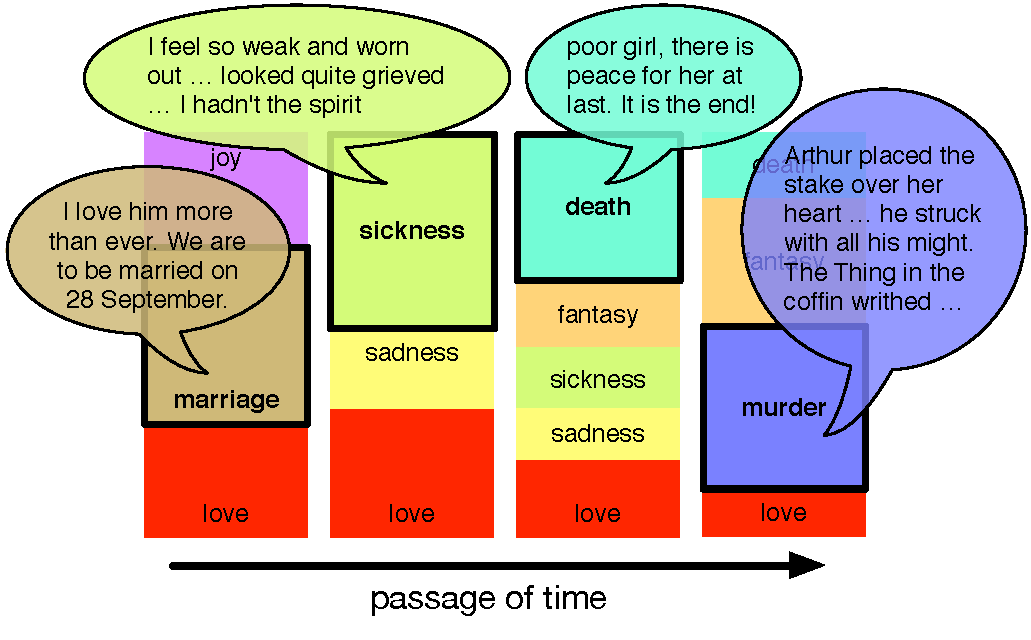
\includegraphics[width=1.0\linewidth]{2016_naacl_relationships/figures/lucy_and_arthur.pdf}
\caption{An example trajectory depicting the dynamic relationship between Lucy
  and Arthur in Bram Stoker's \textit{Dracula}, which starts with love and ends
  with Arthur killing the vampiric Lucy. Each column describes the relationship
  state at a particular time by weights over a set of descriptors (larger
  weights shown as bigger boxes). Our goal is to learn---without
  supervision---both the descriptors and the trajectories from raw fictional
  texts.}
\label{fig:traj}
\end{figure}

When two characters in a book break bread, is their meal just a result
of biological needs or does it mean more?
\newcite{goldthwaite-14} argue that this simple interaction reflects
the diversity and background of the characters, while
\newcite{foster-09} suggests that the tone of a meal can portend
either good or ill for the rest of the book. To support such theories,
scholars use their literary expertise to draw connections
between disparate books: Gabriel Conroy's dissonance from his family
at a sumptuous feast in Joyce's \emph{The Dead}, the frustration of
Tyler's mother in \emph{Dinner at the Homesick Restaurant}, and the
grudging respect for a blind man eating meatloaf in Carver's
\emph{Cathedral}.




However, these insights do not come cheap.  It takes years of careful
reading and internalization to make connections across
books, which means that relationship symmetries and archetypes are
likely to remain hidden in the millions of books published every year
unless literary scholars are actively searching for them.

Natural language processing techniques have been increasingly used to
assist in these literary investigations by discovering patterns in
texts~\cite{jockers-13}.  In Section~\ref{sec:related} we review
existing techniques that classify or cluster relationships between
characters in books using a fixed set of labels (e.g., friend or
enemy).  However, such approaches ignore interactions between
characters that lie outside of the established lexicon and cannot
account for the dynamic nature of relationships that evolve through
the course of a book, such as the vampiric downfall of Lucy and
Arthur's engagement in \textit{Dracula} (Figure~\ref{fig:traj}) or Winston Smith's
rat-induced betrayal of Julia in \textit{1984}.

To address these issues, we propose the task of unsupervised
relationship modeling, in which a model jointly learns a set of
\emph{relationship descriptors} as well as \emph{relationship
  trajectories} for pairs of literary characters. Instead of assigning
a single descriptor to a particular relationship, the trajectories
learned by the model are sequences of descriptors as in
Figure~\ref{fig:traj}.











The Bayesian \emph{hidden topic Markov model} (\htmm) of
\newcite{gruber2007hidden} emerges as a natural choice for our task
because it is capable of computing relationship descriptors (in the
form of topics) and has an additional temporal component. However, our
experiments show that the descriptors learned by the \htmm\ are not
coherent and focus more on events or environments (e.g., meals,
outdoors) than interpersonal states like happiness and sadness.

Motivated by recent advances in deep learning, we propose the \emph{relationship
  modeling network} (\rmn), which is a novel variant of a deep recurrent
autoencoder that incorporates dictionary learning to learn relationship
descriptors. We show that the \rmn\ achieves better descriptor coherence and
trajectory accuracy than the \htmm\ and other topic model baselines in two
crowdsourced evaluations described in Section~\ref{sec:experiments}. In
Section~\ref{sec:discussion} we show qualitative results and make connections to
existing literary scholarship.


















